\documentclass[11pt,a4paper]{article}

\usepackage[utf8]{inputenc}
\usepackage[T1]{fontenc}
\usepackage[spanish,es-nodecimaldot]{babel}
\usepackage{amsmath}
\usepackage{graphicx}
\usepackage{float}
\usepackage{geometry}
\usepackage{booktabs}
\usepackage{hyperref}

\geometry{margin=2.5cm}
\graphicspath{
  {../outputs/phase1/}
  {../outputs/phase2/}
  {../outputs/phase3/}
  {../outputs/phase4/}
}

\title{Proyecto 2: Clasificaci\'on de Se\~nales Eco-Ac\'usticas}
\author{CS3061 -- Machine Learning}
\date{\today}

\begin{document}

\maketitle

\begin{abstract}
Se desarroll\'o un flujo experimental para analizar se\~nales eco-ac\'usticas representadas mediante 64 coeficientes MFCC. Se evaluaron t\'ecnicas de reducci\'on de dimensionalidad, clustering no supervisado, clasificaci\'on supervisada y una pol\'itica operacional basada en umbrales de probabilidad. El desempe\~no fue reportado mediante m\'etricas geom\'etricas, F1-score, matrices de confusi\'on y cobertura por zona de decisi\'on.
\end{abstract}

\section{Contexto de datos}
Se utilizaron estrictamente los archivos \texttt{eco\_acoustic\_train.csv} y \texttt{eco\_acoustic\_test.csv}. El conjunto de entrenamiento contuvo 1906 observaciones y el conjunto de prueba contuvo 477 observaciones. Cada observaci\'on fue descrita por 64 caracter\'isticas continuas \texttt{mel\_0}--\texttt{mel\_63}. La variable objetivo fue \texttt{species\_id}, acotada a cinco clases: 10, 12, 17, 18 y 23. Las variables \texttt{recording\_id}, \texttt{songtype\_id} e \texttt{is\_tp} fueron conservadas como metadatos.

\section{Metodolog\'ia y resultados}
\subsection{Reducci\'on de dimensionalidad}
Se analizaron 1906 observaciones de entrenamiento y 477 observaciones de prueba, descritas por 64 coeficientes MFCC continuos. Antes de aplicar los m\'etodos de reducci\'on de dimensionalidad, se estandarizaron las variables \texttt{mel\_0}--\texttt{mel\_63} mediante media cero y varianza unitaria. Esta etapa fue requerida debido a que PCA, t-SNE y UMAP son sensibles a la escala de entrada.

Se ajust\'o PCA completo sobre el conjunto de entrenamiento con el objetivo de estimar la varianza acumulada por componente principal. El umbral de 95\% de varianza acumulada fue alcanzado con 11 componentes. Posteriormente, se calcul\'o una proyecci\'on PCA en dos dimensiones para compararla contra una t\'ecnica de variedades no lineal. En esta ejecuci\'on, la comparaci\'on se realiz\'o con t-SNE 2D, siguiendo una inicializaci\'on basada en PCA cuando el algoritmo lo permiti\'o.

\begin{table}[H]
\centering
\caption{Comparaci\'on cuantitativa de m\'etodos de reducci\'on de dimensionalidad.}
\begin{tabular}{lrrrr}
\hline
M\'etodo & Tiempo (s) & Varianza 2D & Trustworthiness@10 & Corr. distancias \\
\hline
PCA 2D & 0.002 & 0.671 & 0.867 & 0.947 \\
t-SNE 2D & 13.948 & N/A & 0.987 & 0.590 \\
\hline
\end{tabular}
\end{table}

Se observ\'o que PCA proporcion\'o una referencia lineal interpretable mediante varianza explicada y error de reconstrucci\'on, mientras que la t\'ecnica de variedades fue evaluada mediante preservaci\'on local y correlaci\'on de distancias, ya que no dispone de una raz\'on de varianza explicada equivalente. La separaci\'on visual por \texttt{species\_id} fue inspeccionada en el plano bidimensional para identificar posibles agrupamientos naturales entre las cinco clases.


\begin{figure}[H]
\centering
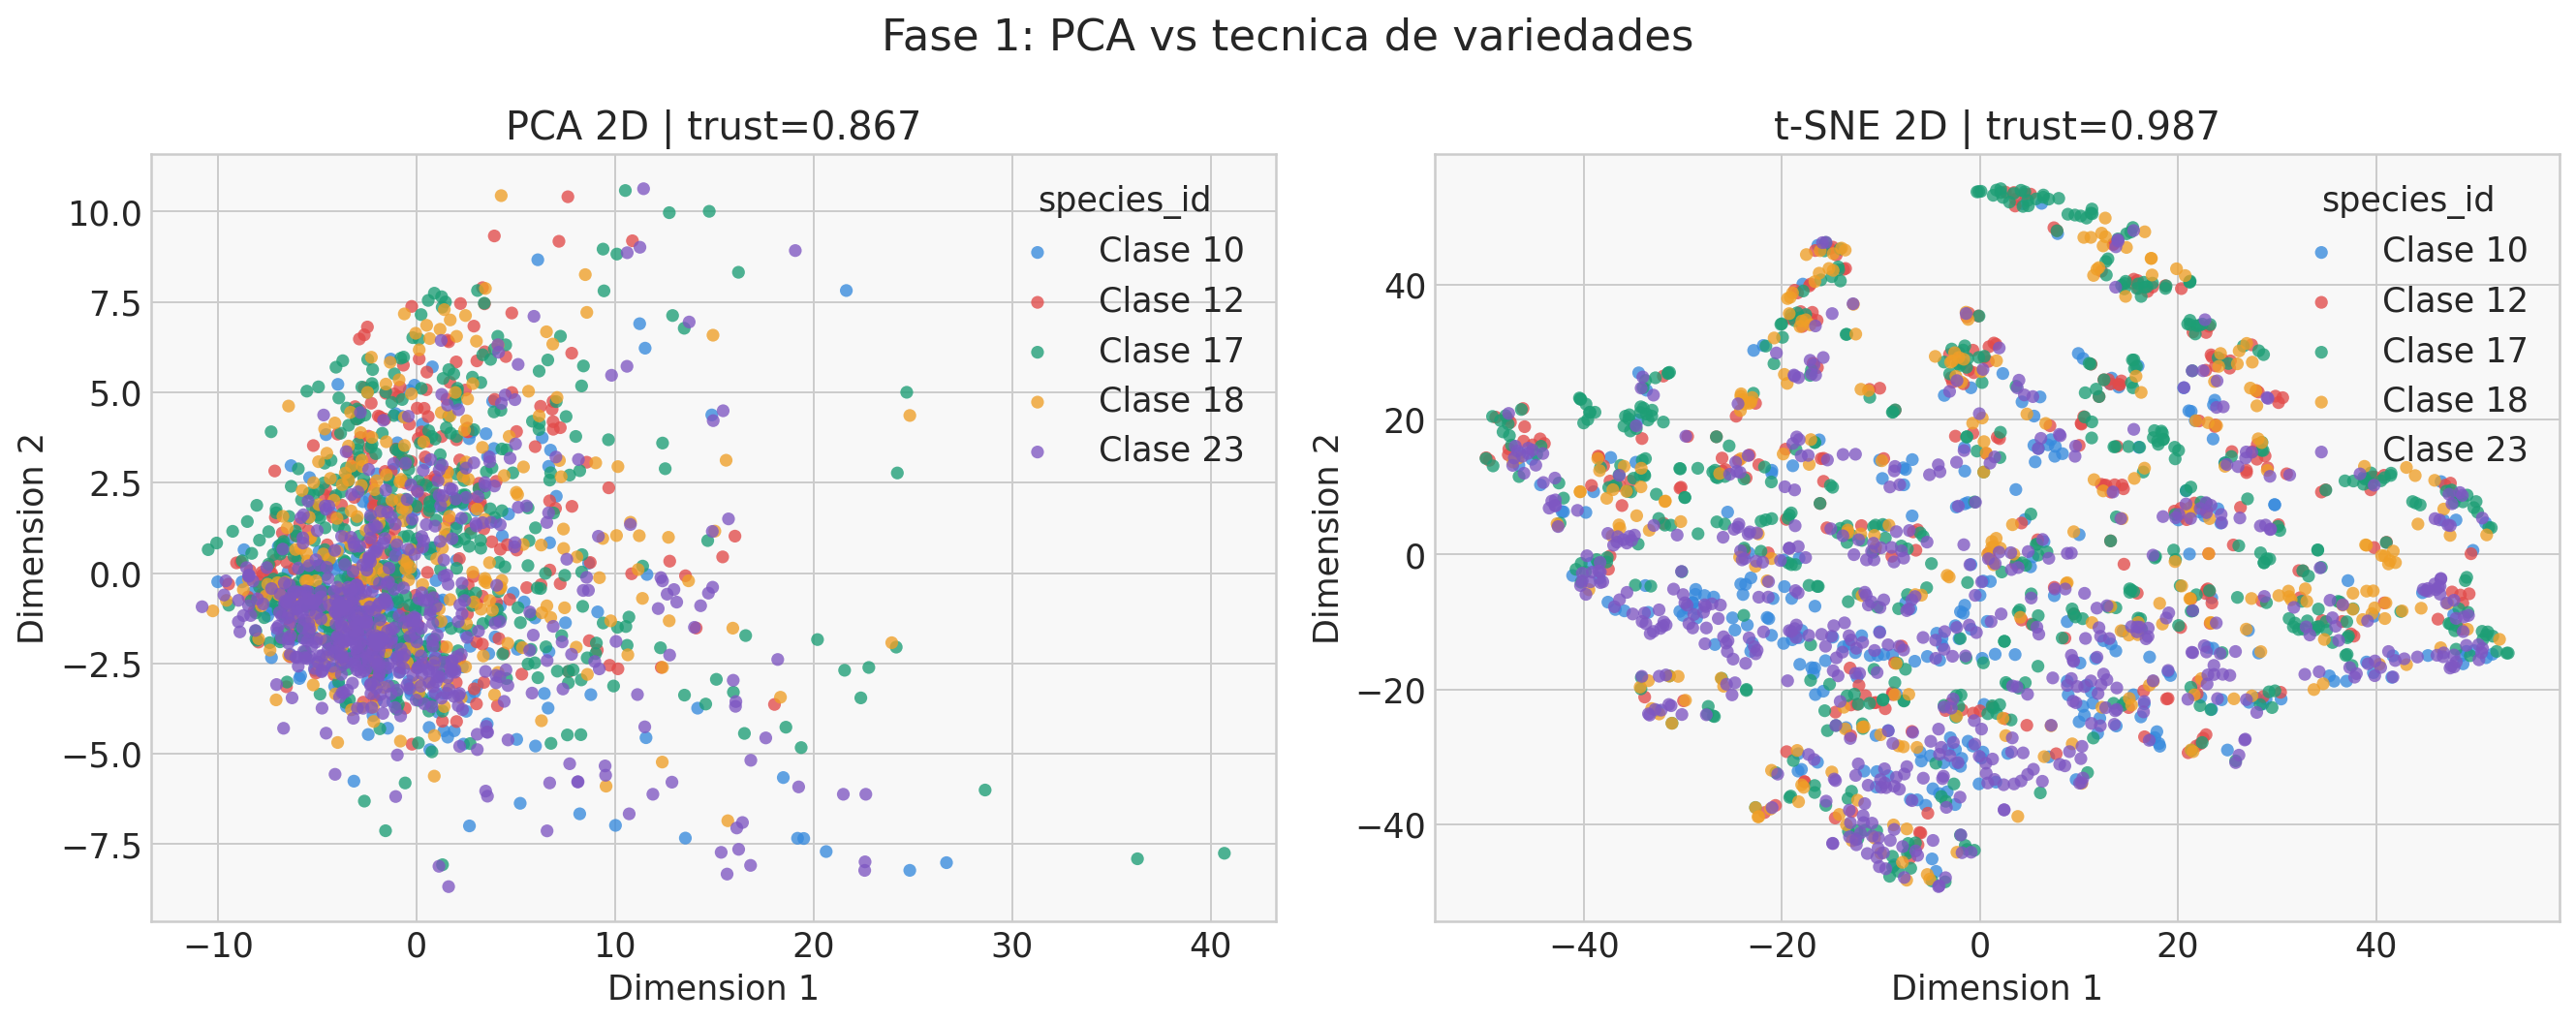
\includegraphics[width=\textwidth]{phase1_embeddings.png}
\caption{Comparaci\'on visual entre PCA 2D y t-SNE 2D.}
\end{figure}

\begin{figure}[H]
\centering
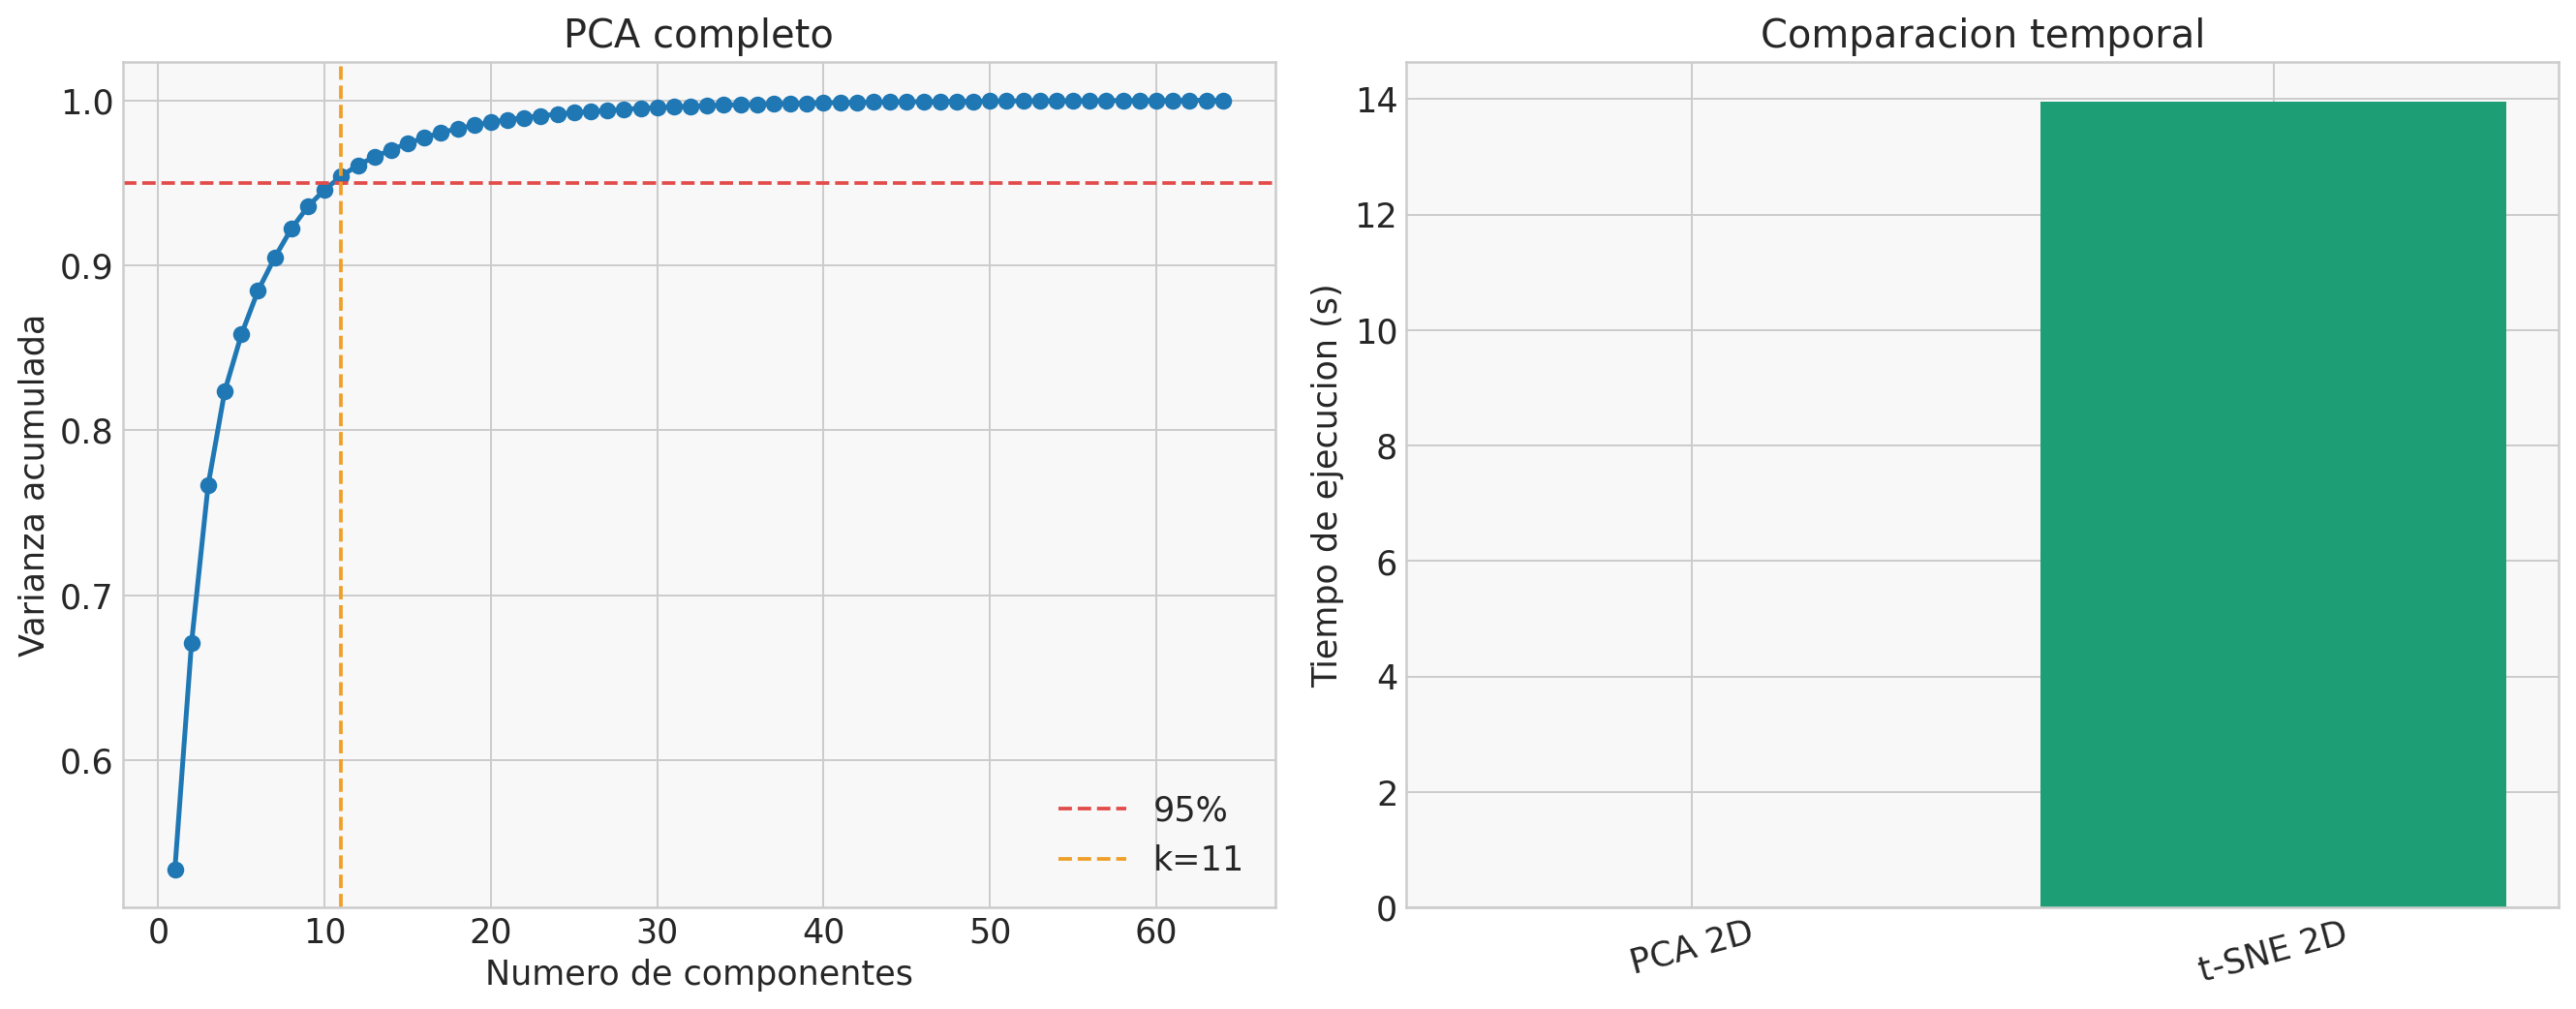
\includegraphics[width=\textwidth]{phase1_diagnostics.png}
\caption{Varianza acumulada de PCA y comparaci\'on temporal.}
\end{figure}

\subsection{Clustering no supervisado}
Se aplicaron dos paradigmas de clustering sobre la representaci\'on PCA que conserv\'o el 95\% de la varianza acumulada. Esta elecci\'on redujo el espacio original de 64 coeficientes MFCC a 11 componentes, con lo cual se mitig\'o el efecto de dimensionalidad alta antes de estimar agrupamientos no supervisados.

Para GMM, se evaluaron valores de $k$ en una grilla discreta y se seleccion\'o el n\'umero de componentes que maximiz\'o el coeficiente de Silhouette. Para DBSCAN, se construy\'o una grilla de $\varepsilon$ a partir de distancias al $k$-\'esimo vecino y se seleccion\'o el radio con mayor Silhouette v\'alida sobre puntos no etiquetados como ruido.

\begin{table}[H]
\centering
\caption{Selecci\'on de modelos de clustering mediante Silhouette.}
\begin{tabular}{lrrrrr}
\hline
M\'etodo & Par\'ametro & Clusters & Silhouette & Ruido & ARI \\
\hline
GMM & k=2 & 2 & 0.184 & 0.000 & 0.026 \\
DBSCAN & eps=4.488, min_samples=10 & 2 & 0.436 & 0.056 & 0.004 \\
\hline
\end{tabular}
\end{table}

El coeficiente de Silhouette fue empleado como criterio geom\'etrico porque compara la cohesi\'on intra-cluster con la separaci\'on inter-cluster mediante $(b-a)/\max(a,b)$. Por tanto, valores m\'as cercanos a uno indicaron particiones con menor solapamiento relativo. El ARI se report\'o solo como diagn\'ostico externo, ya que las etiquetas \texttt{species\_id} no fueron utilizadas para ajustar los modelos de clustering.


\begin{figure}[H]
\centering
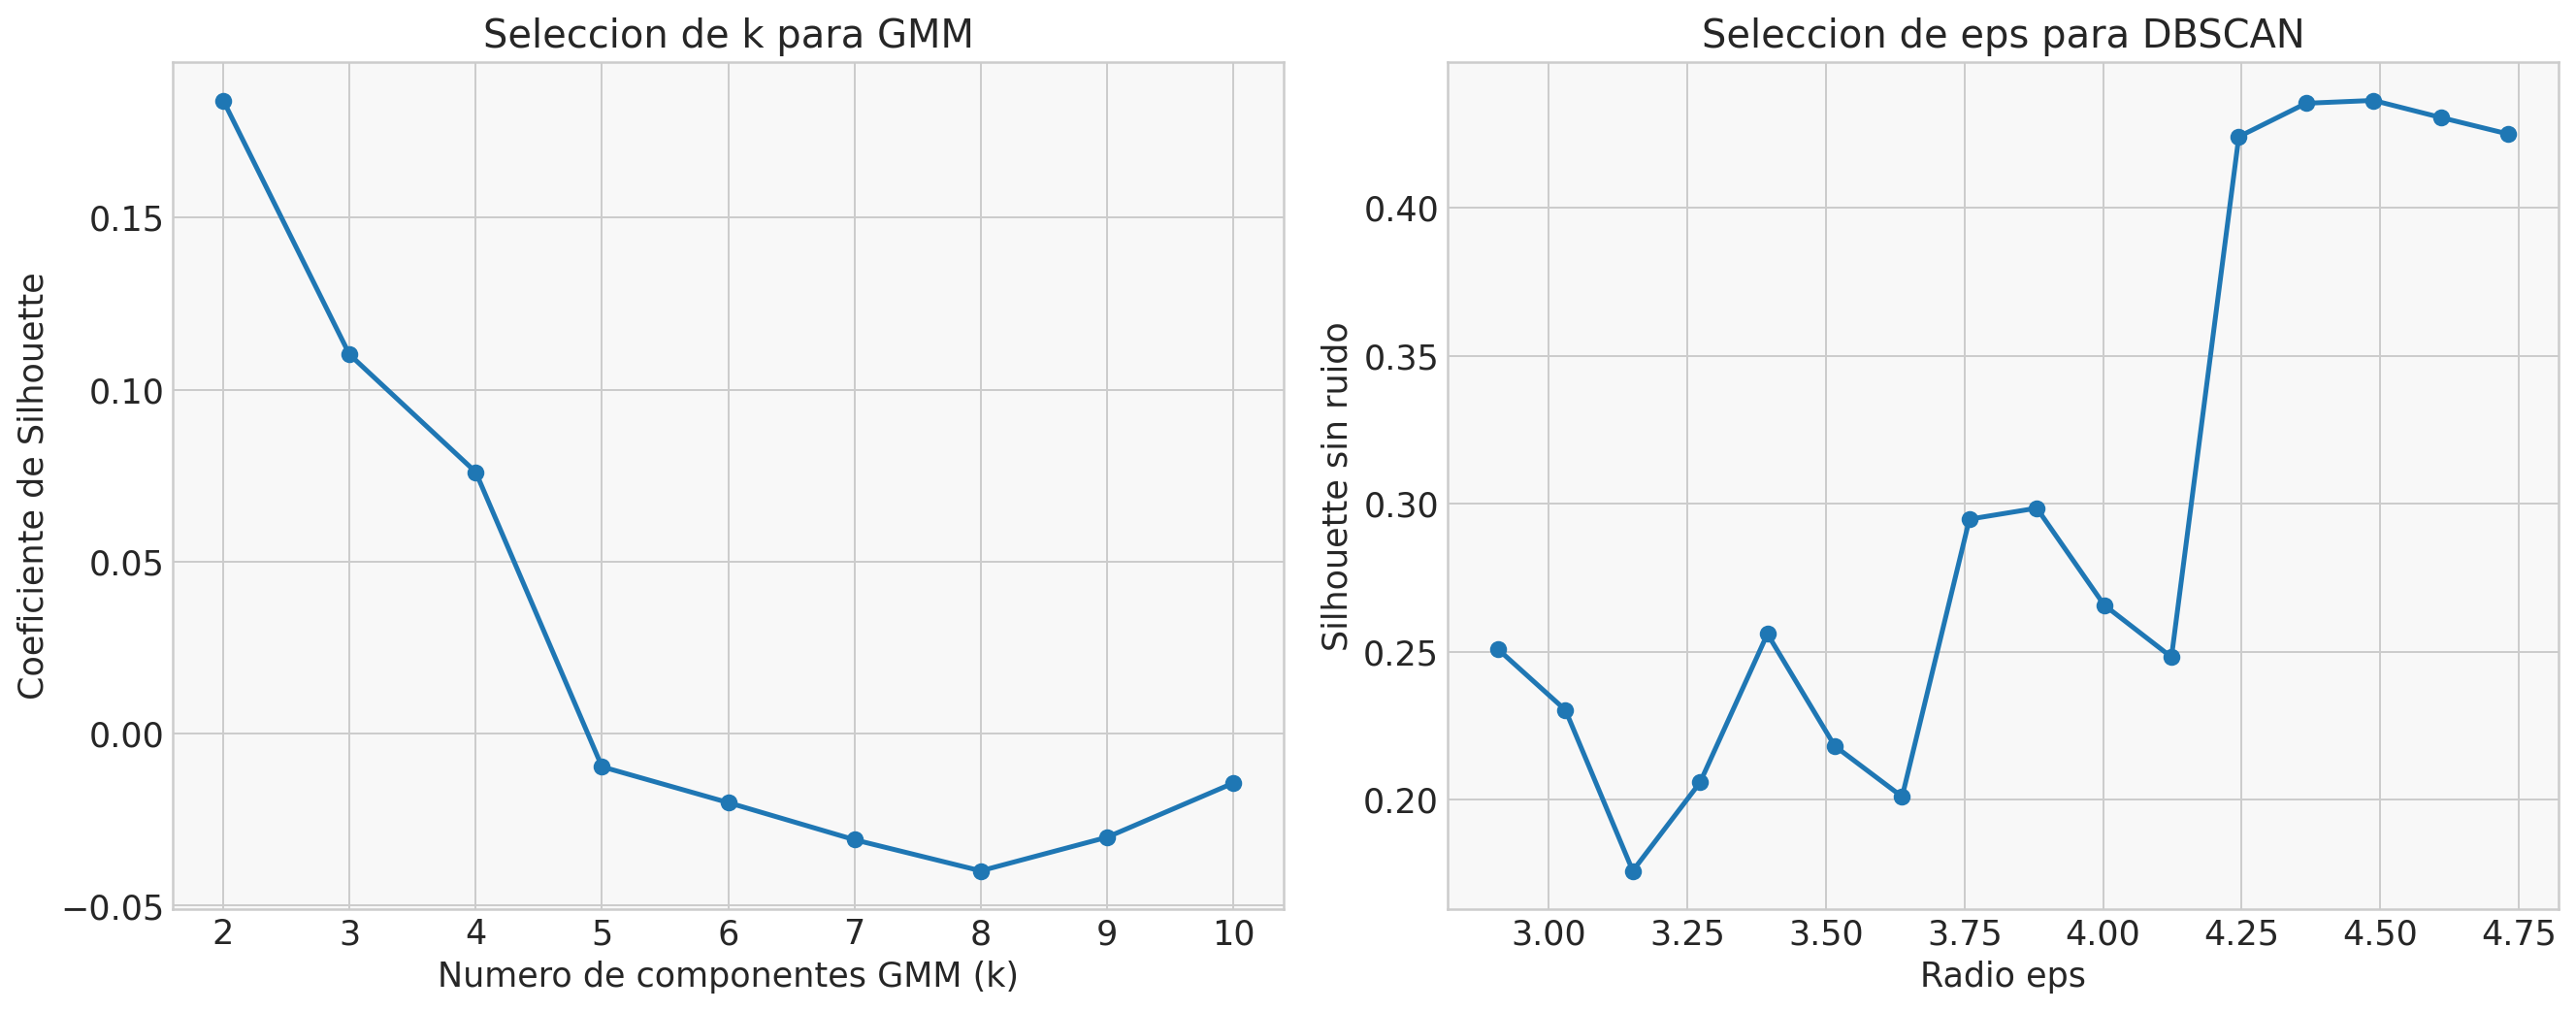
\includegraphics[width=\textwidth]{phase2_silhouette_selection.png}
\caption{Selecci\'on de par\'ametros mediante Silhouette para GMM y DBSCAN.}
\end{figure}

\begin{figure}[H]
\centering
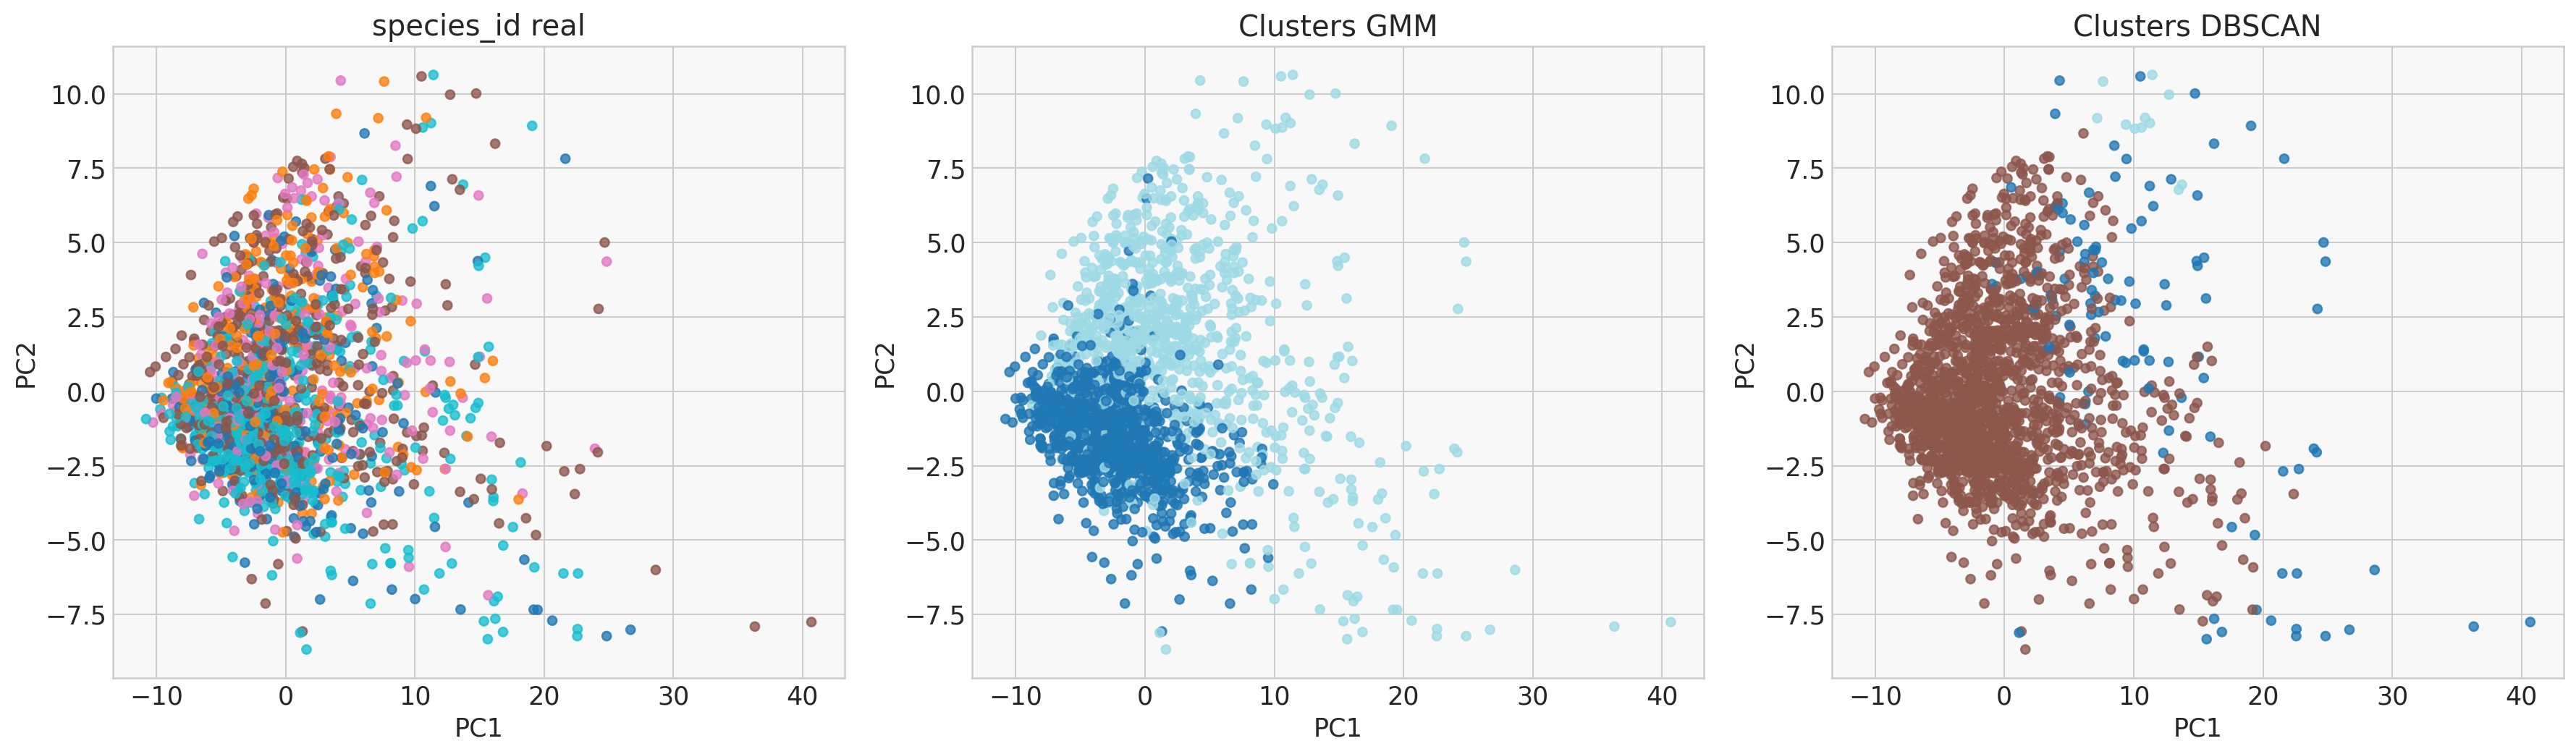
\includegraphics[width=\textwidth]{phase2_clusters_pca2d.png}
\caption{Asignaciones de clustering visualizadas en el plano PCA 2D.}
\end{figure}

\subsection{Clasificaci\'on supervisada}
Se entrenaron dos modelos supervisados sobre los 64 coeficientes MFCC estandarizados. El primer modelo correspondi\'o a una red MLP implementada en TensorFlow/Keras con topolog\'ia $64 \rightarrow 128 \rightarrow 64 \rightarrow 5$. En las capas ocultas se aplicaron Batch Normalization, activaci\'on ReLU y Dropout con tasas 0.30 y 0.20, respectivamente. La funci\'on de p\'erdida utilizada fue entrop\'ia cruzada categ\'orica dispersa, optimizada mediante Adam.

El segundo modelo correspondi\'o a un ensamble por votaci\'on suave compuesto por Random Forest, Extra Trees e HistGradientBoosting. Se utilizaron probabilidades posteriores estimadas por cada componente y se agregaron mediante votaci\'on probabil\'istica. La red neuronal fue entrenada durante 69 \'epocas efectivas con parada temprana.

\begin{table}[H]
\centering
\caption{Desempe\~no de componentes del ensamble en validaci\'on.}
\begin{tabular}{lrr}
\hline
Modelo & F1 ponderado validaci\'on & Tiempo (s) \\
\hline
random_forest & 0.443 & 2.471 \\
extra_trees & 0.422 & 1.326 \\
hist_gradient_boosting & 0.422 & 13.987 \\
soft_voting_ensemble & 0.437 & 16.853 \\
\hline
\end{tabular}
\end{table}

\begin{table}[H]
\centering
\caption{Comparaci\'on de clasificadores sobre el conjunto de prueba.}
\begin{tabular}{lrrr}
\hline
Modelo & Accuracy & F1 macro & F1 ponderado \\
\hline
MLP TensorFlow & 0.451 & 0.451 & 0.450 \\
Soft Voting Ensemble & 0.491 & 0.428 & 0.469 \\
\hline
\end{tabular}
\end{table}

El F1-score fue priorizado porque el problema contiene cinco especies y la distribuci\'on de clases puede inducir diferencias entre desempe\~no global y desempe\~no por clase. Las matrices de confusi\'on permitieron inspeccionar errores de asignaci\'on entre especies ac\'usticamente cercanas, mientras que las curvas de aprendizaje permitieron controlar el sobreajuste asociado a la red neuronal.


\begin{figure}[H]
\centering
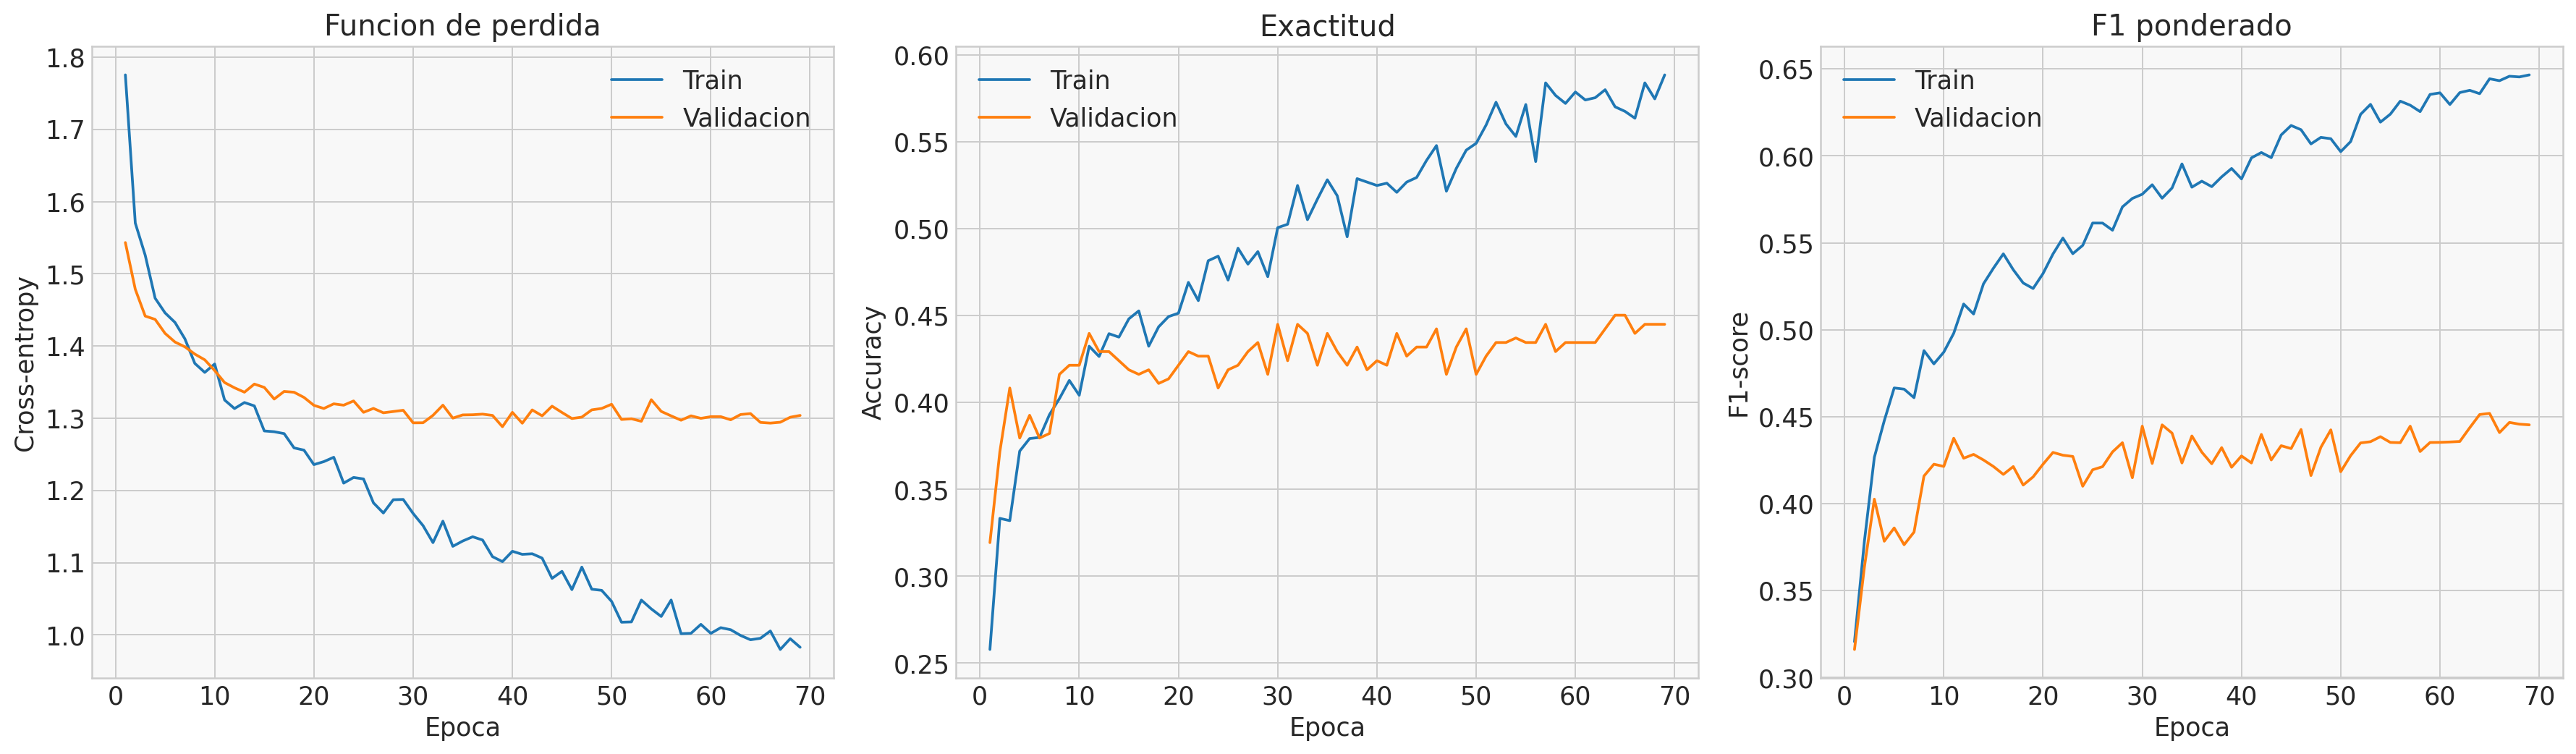
\includegraphics[width=\textwidth]{phase3_mlp_learning_curves.png}
\caption{Curvas de aprendizaje del MLP con Batch Normalization y Dropout.}
\end{figure}

\begin{figure}[H]
\centering
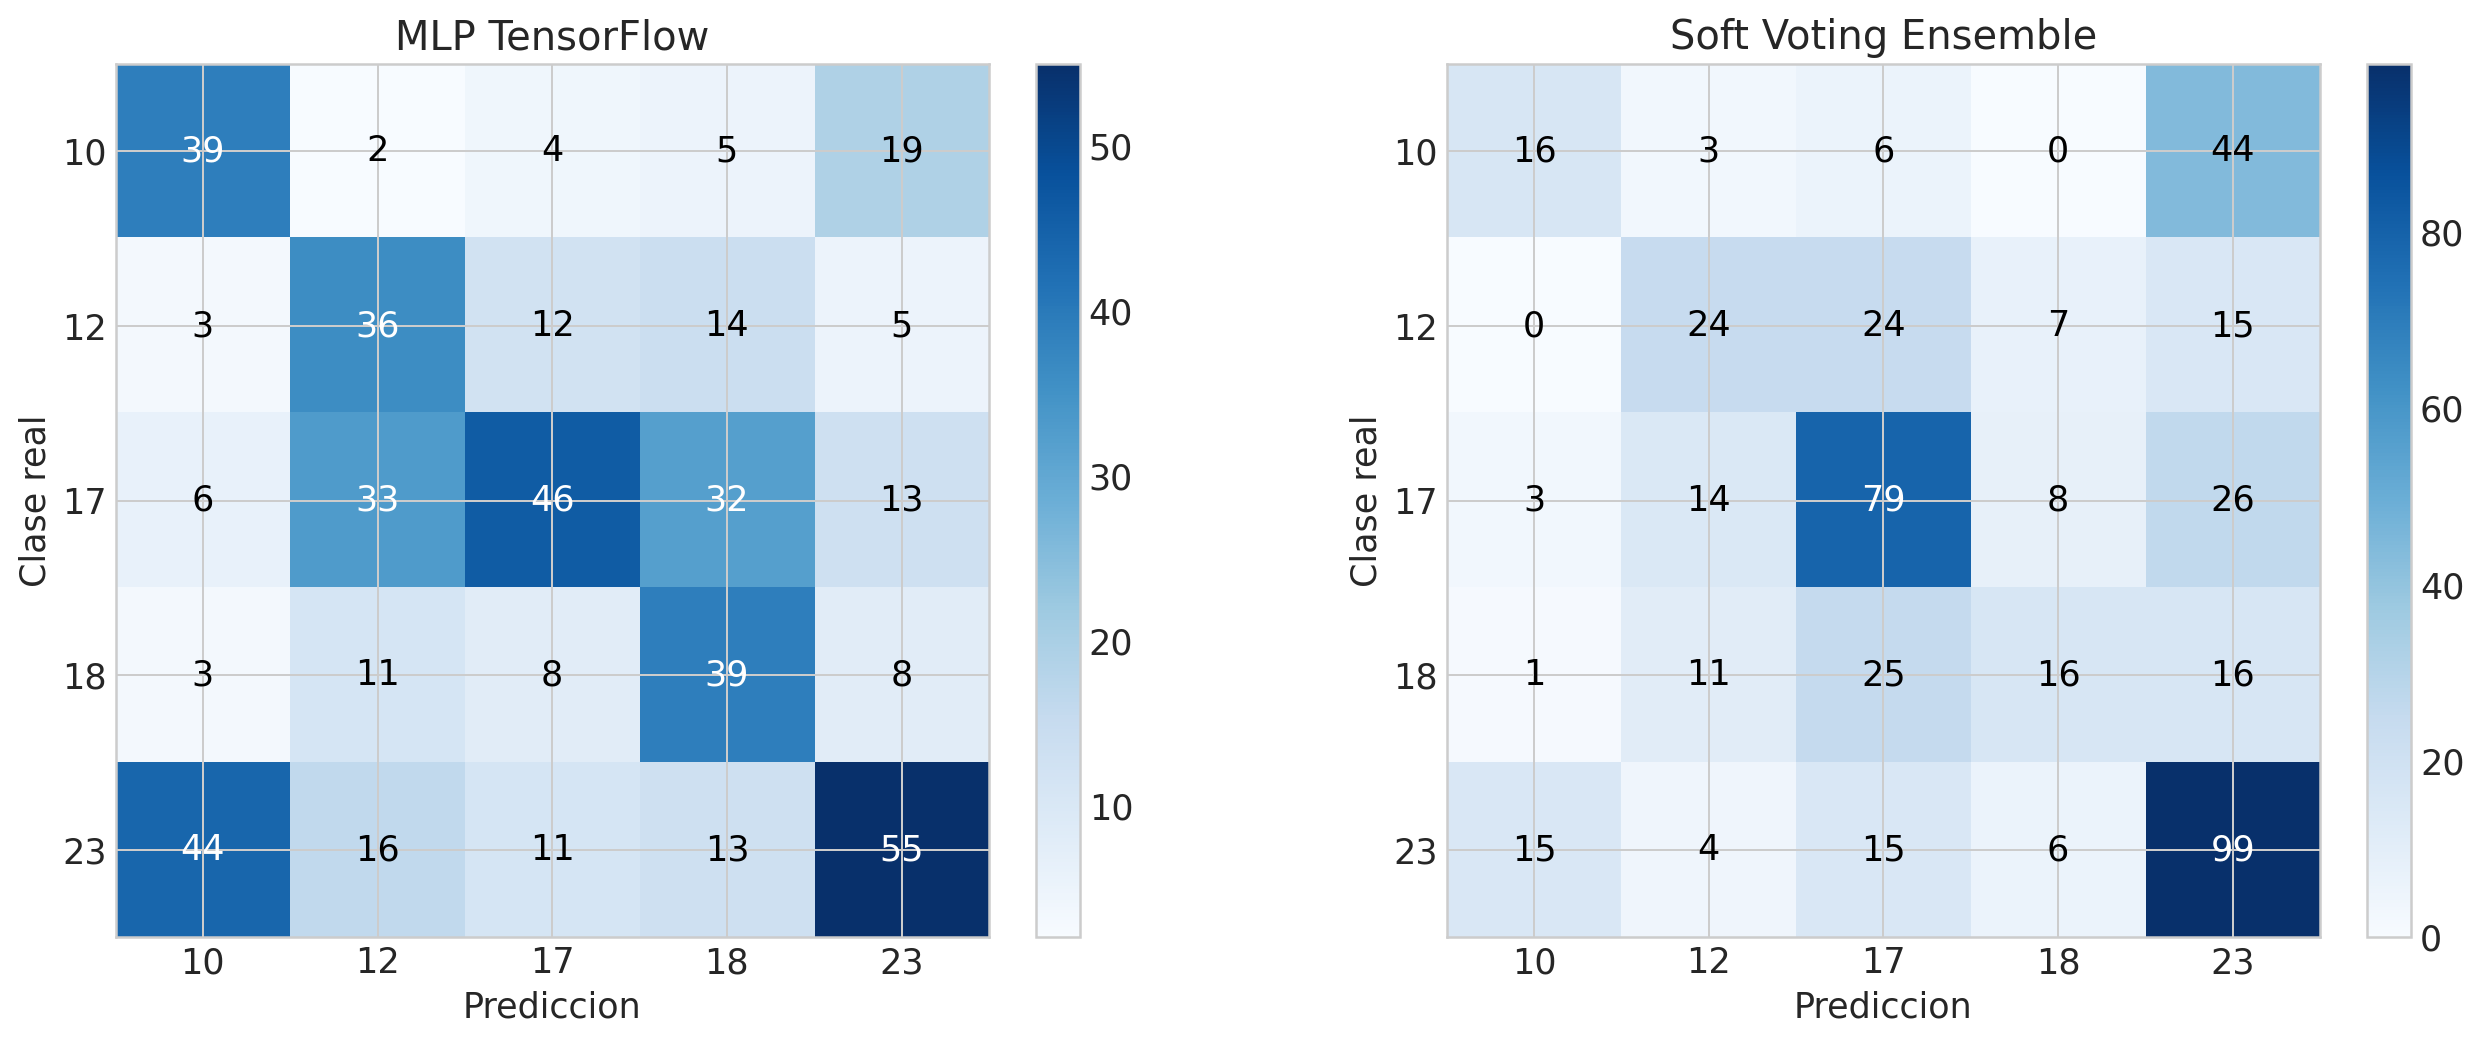
\includegraphics[width=\textwidth]{phase3_confusion_matrices.png}
\caption{Matrices de confusi\'on de los modelos supervisados.}
\end{figure}

\subsection{MLOps y l\'ogica de umbrales}
Se propuso una pol\'itica operacional basada en la probabilidad posterior m\'axima del modelo Soft Voting Ensemble. Las predicciones con $P \geq 0.85$ fueron asignadas a la zona de confianza, las predicciones con $0.40 \leq P < 0.85$ fueron asignadas a la zona de incertidumbre y las predicciones con $P < 0.40$ fueron asignadas a la zona de rechazo.

\begin{table}[H]
\centering
\caption{Resumen operativo de zonas de decisi\'on.}
\begin{tabular}{lrrrr}
\hline
Zona & Observaciones & Cobertura & Accuracy & Prob. media \\
\hline
Zona de Confianza & 9 & 0.019 & 0.667 & 0.883 \\
Zona de Incertidumbre & 417 & 0.874 & 0.492 & 0.588 \\
Zona de Rechazo & 51 & 0.107 & 0.451 & 0.353 \\
\hline
\end{tabular}
\end{table}

La zona de confianza fue definida para automatizar decisiones de clasificaci\'on con alta certeza. La zona de incertidumbre fue destinada a revisi\'on humana o validaci\'on secundaria, mientras que la zona de rechazo fue reservada para casos donde no deber\'ia emitirse una clasificaci\'on autom\'atica. Esta l\'ogica permite controlar el riesgo operativo al separar cobertura del sistema y confiabilidad de las decisiones aceptadas.


\begin{figure}[H]
\centering
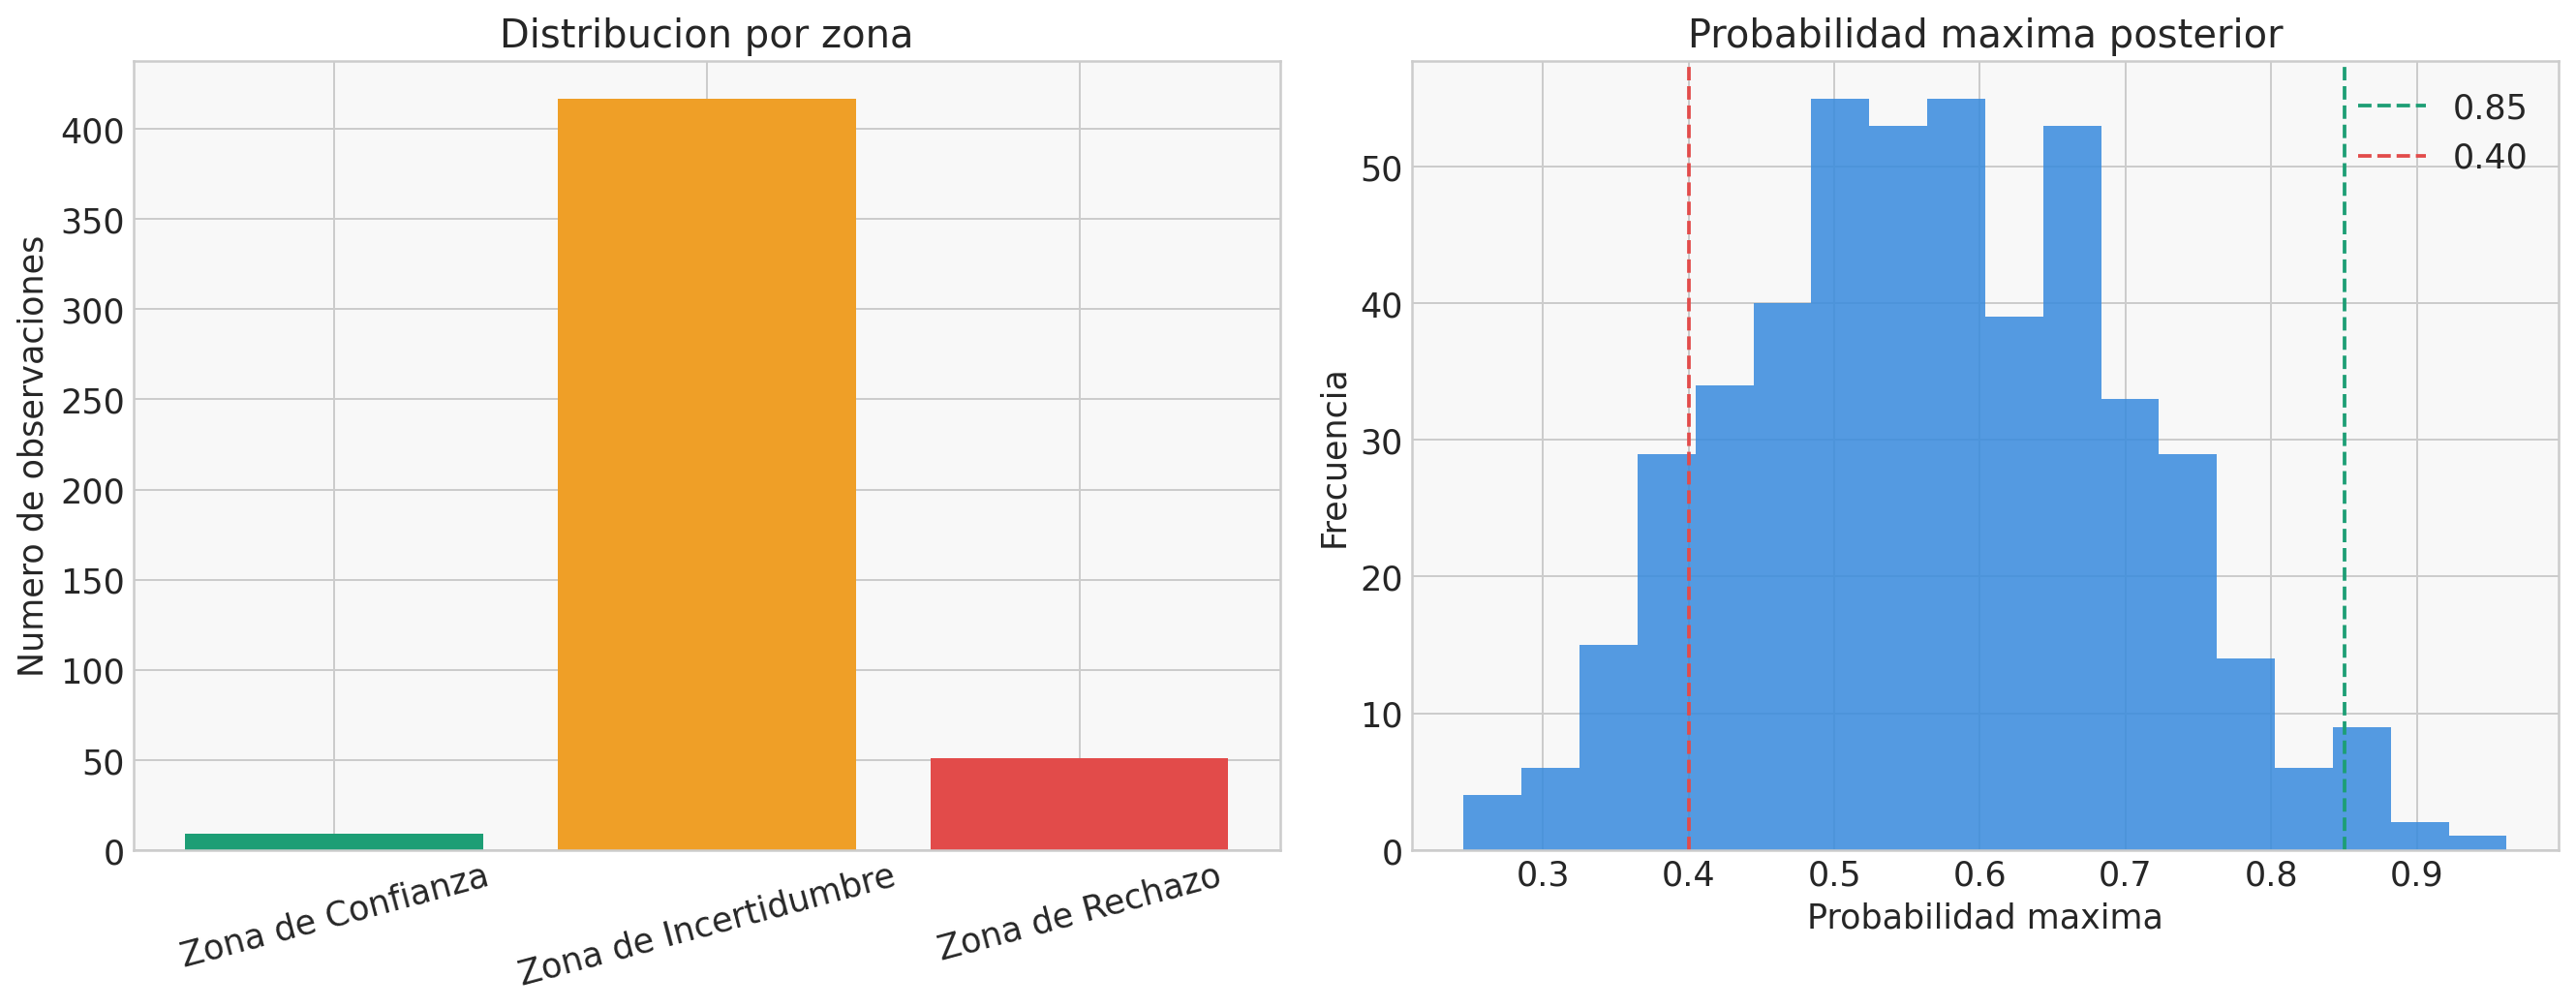
\includegraphics[width=\textwidth]{phase4_threshold_diagnostics.png}
\caption{Distribuci\'on de zonas y probabilidades posteriores m\'aximas.}
\end{figure}

\section{Discusi\'on}
Se evidenci\'o que la representaci\'on lineal PCA preserv\'o una proporci\'on importante de la estructura global, mientras que t-SNE preserv\'o mejor vecindarios locales. En clustering, los agrupamientos geom\'etricos no coincidieron de forma fuerte con las especies reales, lo cual sugiri\'o solapamiento ac\'ustico entre clases o dependencia de factores no incluidos en los MFCC. En clasificaci\'on supervisada, el ensamble por votaci\'on suave super\'o ligeramente al MLP en F1 ponderado sobre el conjunto de prueba.

\section{Conclusiones}
Se implement\'o un pipeline reproducible para reducci\'on de dimensionalidad, clustering, clasificaci\'on y umbralizaci\'on probabil\'istica. El resultado indic\'o que la clasificaci\'on autom\'atica debe ser empleada con control de incertidumbre, debido a que la mayor proporci\'on de observaciones qued\'o ubicada en la zona intermedia de probabilidad. Se recomend\'o utilizar la zona de confianza para automatizaci\'on conservadora y reservar la zona de incertidumbre para revisi\'on experta.

\end{document}
